
\documentclass[12pt,oneside,a4paper]{article}
%
\usepackage{graphicx}
\usepackage{tabularx}
\usepackage{url}
\usepackage[latin1]{inputenc}
%\usepackage[utf8]{inputenc}
\usepackage[left]{eurosym} 
\usepackage{times}
\usepackage{pdfpages}
\usepackage{todonotes}
\usepackage{enumerate}

% We don't want a special font for urls (looks bad with times):
\urlstyle{same}

% Graphics extensions and path:
%\DeclareGraphicsExtensions{.pdf,.png,.jpg}
%\DeclareGraphicsExtensions{.eps,.ps}
%\graphicspath{{figures/}}

%
% Page size
%
\usepackage[top=25mm,left=25mm,right=25mm,bottom=25mm]{geometry}

\setlength{\headheight}{15pt}    % Necessary to avoid fancyhdr warning.


\newcommand\LongTitle{Humidity, clouds and snow in the Arctic}
\newcommand\ShortTitle{Humidity, clouds and snow in the Arctic}



%
% Heading
%
\newcommand{\pagevers}[2]{
\ifnum\thepage=1 
#1
\else#2
\fi
}
%
\usepackage{fancyhdr}
\pagestyle{fancy}
\chead{}
%\rhead{\pagevers{}{\bf \thepage}}
\rhead{\thepage}
\rfoot{\small \it \ShortTitle\ ---\  Application to SNSA 2021-R}
\cfoot{}
\lfoot{}
%\renewcommand{\headrulewidth}{\pagevers{0pt}{0.2pt}}
\renewcommand{\headrulewidth}{0.2pt}
\renewcommand{\footrulewidth}{0pt}


\newcommand{\docname}[1]{\lhead{\small #1}}

%
% Section titles
%
\usepackage[small]{titlesec}
\titlespacing*{\section}{0pt}{*3.3}{*0.5}
%
% 
%
\def\compactitems{\parskip0pt\topsep0pt\partopsep0pt\parsep0pt\itemsep0pt}

% Struts for better table formatting:
\newcommand\T{\rule{0pt}{2.6ex}}
\newcommand\B{\rule[-1.2ex]{0pt}{0pt}}


\newcommand{\FIXME}[1]{{\bfseries \textcolor{red}{FIXME:} #1}}
\newcommand{\md}[1]{\mbox{#1-d}}
%\newcommand{\3d}{3d}

%\hyphenation{3-d}
\uchyph=0

%%% Local Variables: 
%%% mode: latex
%%% TeX-master: t
%%% End: 



\docname{Project description}
\usepackage{graphicx}
\usepackage{caption}
\usepackage{subcaption}
\usepackage{multirow}
\captionsetup[figure]{font=normalsize,labelfont=normalsize}

%
% References
%
\usepackage{natbib}
\bibliographystyle{agu04}     
\setlength{\bibsep}{0mm}


\newcommand\wpstart[3]{\noindent\textbf{WP #1, #2}\hspace{\stretch{1}}Priority #3%
	\vspace{-4mm}\\\rule{\textwidth}{0.5pt}\\}
\newcommand\wpenda[4]{%
	\noindent -----\\ 
	\begin{tabularx}{0.95\hsize}{l p{133mm}}    
		\hspace*{-1.1ex}Start\,--\,end: & #1\\
		\hspace*{-1.1ex}Main output: & #2\\
		\hspace*{-1.1ex}Main risks: & #3\\
	\end{tabularx}\\
	\vspace{-2.2ex}\noindent\rule{\textwidth}{0.5pt}\\
}


\begin{document}
	
	
	\thispagestyle{empty}
	\vspace*{-10mm}
	\noindent
	\textbf{\Large \LongTitle}




\section{General summary}

Water vapour plays an important role in the water and energy cycle over the polar regions, especially over Arctic. Over the Arctic, changes in the water vapour content are most sought to observe the warming trends, also known as Artic amplification. However over poles, the ground measurements are sparse and the performance of the satellite retrievals is constrained by the highly variable surface emissivity. The basic aim of this project is to develop new retrieval algorithms principally for total water vapour (TWV) from satellite microwave radiometer data over the Arctic. We propose a physically based retrievals, using a Bayesian machine learning based inversion method. Additionally, this algorithm could be used to also retrieve side products like total liquid water content (LWC) and sea-ice concentration (SIC). A key feature of this algorithm would be the use high resolution SAR imagery to classify sea-ice and open waters. Fine scale sea-ice information is necessary for distinguishing emissivity between different surface types. Another crucial aspect of the development line will be to use data from multiple microwave frequencies, with different footprint size, and avoiding the remapping of data. The overall scheme shall be similar to the one in a parallel SNSA 2021 proposal submitted by co-applicant Patrick Eriksson.
The resulting dataset would play an important role in not only analysing the water vapour variability of the Arctic atmospheric but also in deciphering the trends the Arctic climate change.


\subsection{Background}
%
\label{sec:background}
Some info from Luisa (1/2 page)

\subsection{Previous works}
%
\label{sec:previousworks}
Accurate measurements of water vapour profile over polar regions is through ground based microwave radiometers or radiosondes. For a comprehensive overview as required for monitoring purposes can only be achieved through space borne observations. However, over polar regions, the main challenge encountered by microwave (MW) observations based retrieval algorithms is the high and highly variable surface emissivity which dominates the signal. The most important work towards retreival of WVP from microwave humidity sounders (such as Advanced Microwave Sounding Unit-B (AMSU-B) and Microwave Humidity Sounder (MHS)) comes from University of Bremen. Their retrieval concept was initiated by \citet{miao:2001:atmos}, where they utilized water vapour absorption channels around 183\,GHz and  150\,GHz window channel to retrieve total water vapour (TWV) upto 7\,kg m$^{-2}$. Subsequently in the study \citep{} they extended this approach to include 89\,GHz to retrieve TWV upto 15\,kg m$^{-2}$ over sea-ice regions and formulated a relationship between sea-ice emissivity over different frequencies using measurement campaigns. Later, \cite{scarlat:2018:retri} extended the method to include all surface types using AMSU-B. A comparison of the retrieved WVP against ERA-Interim showed that the over winter months, the RMSD was  1.86\,kg m$^{-2}$ but over summer months the errors were up to 5.67 m$^{-2}$ due to the algorithm being constrained by its upper retrieval limit of 15 m$^{-2}$. Besides MW sounding, an attempt at TWV has also been made using low frequency microwave observations from Advanced Microwave Scanning Radiometer (AMSR). For example, \citet{scarlat:2017:exper} use optimal estimation (OEM) for multi-parameter retrieval over Arctic, and \citet{zabolotskikh:2020:anadv} attempt at TWV retrieval over both open ocean and sea-ice regions using neural networks based inversion. In both products, the highest uncertainties in the retrieval are linked to the empirical estimates of surface emissivity over sea-ice regions.


The lack of an accurate atmospheric data over the extensive Arctic sea-ice regions has implications in the forecast skill of numerical weather prediction (NWP) models. Though the  models are themselves suffer from limitations associated with the modelling of snow, sea ice, mixed-phase clouds, \citet{lawrence:2019:usean} show that MW sounding observations have a clear positive impact on the predictive skill in the summer months. Over the winter months the optimal utilisation of the observations is constrained by the presence of snow and sea-ice. Infact,  increasing the usage of satellite data over all surfaces in Integrated Forecast System (IFS) is identified as one of the priorities in ECMWF Strategy for 2021-2030. 


\subsection{The way forward}

\subsubsection{Problems and solutions}

Remote sensing provides indirect measurements and the data retrieval always
offers some degree of complexity. When using passive satellite microwave data
to estimate humidities over the Arctic region, the main limiting factor is the
surface's contribution to measured radiances. The special role of the surface
is due to high atmospheric transmissivities and the difficulties to predict the
surface properties of snow (on either land or ice). The main solution today is
to reject channels with a significant surface contribution. This gives a low
utilisation rate of the satellite data, and leaves the humidity close to the
surface unconstrained.

For this reason, efforts are being made to improve the "forward modelling",
i.e.\ use auxiliary data to predict the local radiative properties of snow. This
constitutes a very hard problem as the properties depend on a high number of
snow variables. There will be progress in the area, but it will likely be slow.
There is also another, less discussed, consideration, that the satellite
footprint can cover both sea ice and open water. To handle this, a large scale
ice-fraction is not sufficient, even the distribution of ice and water inside
the footprint matters. That is, retrievals above leads are particularly
problematic. The risk of having an inhomogeneuos footprint increases with
footprint size, and good spatial resolution is thus advantageous even if the
atmospheric fields show little horizontal variability.

We will attack these issues from a new angle, now feasible due to progress in
machine learning (ML). We avoid the limitations in traditional approaches by
basing the inversions on a retrieval database, that is used to train the ML
model. The simulated observations in the database are generated on
high-resolution data and variations of both surface and atmospheric variables
inside the footprint get included. In addition, by simulating "scenes" of
adjacent footprints, and not just individual ones, the information hidden in
the overlap of footprints can be exploited. The later effectively increases the
horizontal resolution, but also provides background spatial information, such
as indications on if the surface is homogeneous or mixed.


\subsubsection{Some clarifications}

The ML approach to be applied is introduced by us and operates in a Bayesian
manner. Most importantly, it provides robust case specific error estimates.
That is, an uncertainty is assigned to each individual retrieval.

The database works like the prior assumptions in a standard Bayesian retrieval,
but by using ML we are not restricted to Gaussian statistics, can handle
strongly non-linear problems, and we can include aspects that are very
difficult to handle in traditional retrievals (such as inhomogeneuos
footprints). It is not needed to predict the conditions exactly where the
observation is made, it suffices that simulations have a similar variability as
reality. The ML algorithm uses the database provided to give the posterior
knowledge of the quantity sought, given the scene of observations.

If useful additional information can be provided, this can be incorporated in
the ML training. For example, if there is progress in snow modelling and the
local emissivity can be estimated with some certainty, this can be seen as a
virtual measurement and be used to improve the ML model.



\section{Project description}

The retrieval of atmospheric parameters from brightness temperatures is an inverse problem. The Bayesian retrieval methods provide a way to handle the ill-posedness of the retrieval problem and its associated uncertainties. In this project, we utilize  Quantile Regression Neural Network (QRNN), a machine learning technique to invert the simulated brightness temperatures (TB) to WVP. The database with simulated TB profiles is generated using Atmospheric Radiative Transfer Simulator (ARTS). 
 
\subsection{Satellite instruments}
This scheme developed here would not only be applicable to existing conical radiometers like  Special Sensor Microwave Imager/Sounder (SSMIS) and cross-track radiometers e.g.\, Advanced Technology Microwave Sounder (ATMS); but also the upcoming satellite instruments like Arctic Weather Satellite (AWS) and MicroWave Imager (MWI). The project can also be termed as preparatory step towards operational use of AWS data. Table~\ref{tab:instruments} gives a brief description of the satellite instruments which are relevant to this study. 

\begin{table}[t]
	\caption{Specifications of satellite instruments relevant to this study.}
	\label{tab:specifications_instruments}	
	\begin{tabular}{rrr}

		Instruments & Frequency range 	& Resolution  \\
					& [GHz]				& [km]			\\
		\hline			
		SSMIIS		&

		\hline			

	\end{tabular}
\end{table}

 
\subsection{Tools}
\subsubsection{QRNN}
%
\label{sec:qrnn}
The neural network (NN) training is a process of learning to predict the outputs {$y_i$} from inputs {$x_i$} through a series of learnable transformations. In traditional NN techniques, the output is a point estimate of the target variable. However, QRNN is trained to minimise the mean of the quantile loss function and predict chosen quantiles of its Bayesian a posterior distribution. QRNN can be seen as a machine learning version of Bayesian Monte Carlo integration (BMCI) to solve ill-posed problems. A detailed description of QRNN can be found in \citet{pfreundschuh:aneur:18}.  

In all the applications QRNN has been tested so far, it has outperformed the existing approaches. This includes a very recent study by the main applicant for predicting clear noise-free clear-sky radiances from microwave humidity channels \citep{kaur:2021:canma}. Previously, \citet{pfreundschuh:aneur:18} had shown the advanatge of QRNN in predicting cloud top pressure from observations by the Moderate Resolution Imaging Spectroradiometer (MODIS). Recent studies with QRNN also include working with GPROF team  to replace BMCI by QRNN for GPROF retrievals (manuscript in preparation).


\subsubsection{ARTS}
\label{sec:arts}
% 
The backbone of our work is buliding the database with simulated TB using ARTS (Atmospheric Radiative Transfer Simulator, \url{www.radiativetransfer.org}). ARTS has some unique features, but in this context it is rather the completeness and flexibility of ARTS that is
helpful. There is now a second cornerstone of the ARTS infrastructure, the
associated database of single scattering properties \citep{eriksson:agene:18}.
The main part contains data for 36 particle ``habits'' assuming totally random
orientation (TRO). Already this makes the database the most comprehensive one.
Some data for azimuthally random orientation (ARO) are also at hand
\citep{brath:micro:20,ekelund:micro:20}. In principle more ARO data of ice
hydrometeors are needed, but in \citet{baralakas:intro:21} we show that the ARO
case can be fairly well approximated by scaling TRO data. In an ongoing master
thesis project data for melting particles are being generated, and this then
fills the main remaining gap in the database.

\subsection{Preliminary results}
%
This project will build up on the ongoing efforts, hence we shall briefly summarize the preparatory steps we have undertaken to demonstrate the feasibility of the project. 

\subsubsection{Radiative transfer simulations}
%
Towards creating as realistic and comprehensive retrieval databases as possible, we prepare for the complex radiative transfer calculations using the Global Precipitation Measurement (GPM) Microwave Imager (GMI) frequencies and polarisations. GMI provides observations upto 65$^{\circ}$ and is used as a baseline to formulate the full range of atmospheric and oceanic conditions, including snow and sea-ice emissivities over higher latitudes. The GMI measurements for frequencies around 166\,GHz and 183\,GHz are simulated using Cloudsat radar measurements. A dbZ based systems as described by \citet{ekelund:using:20} is followed and onion peeling retrieval method is used to invert CloudSat reflectivities to Ice Water Content (IWC). The emissivity over land and water are taken from Tool to Estimate Land-Surface Emissivities at Microwave frequencies \citep{aires} and Tool to Estimate Sea-Surface Emissivity from Microwaves to sub-Millimetre waves \citep{prigent}. However for snow and sea-ice surface types, experimental and modelling studies \citep{harlow:2009:milli, harlow:2012:tundr,hewison:2002:airbo} are used to define the valid ranges of emissivity variability for 166\,GHz and 183 \,GHz frequencies. Differences between H and V polarisation are also taken into account. For each snow/sea-ice observation (identified using ERA5), the corresponding emissivity is set randomly within the ranges of variability.

\subsubsection{Training database}
%
\begin{figure*}[t]
	\centering
	\begin{subfigure}{.24\textwidth}
		\caption{Land}
		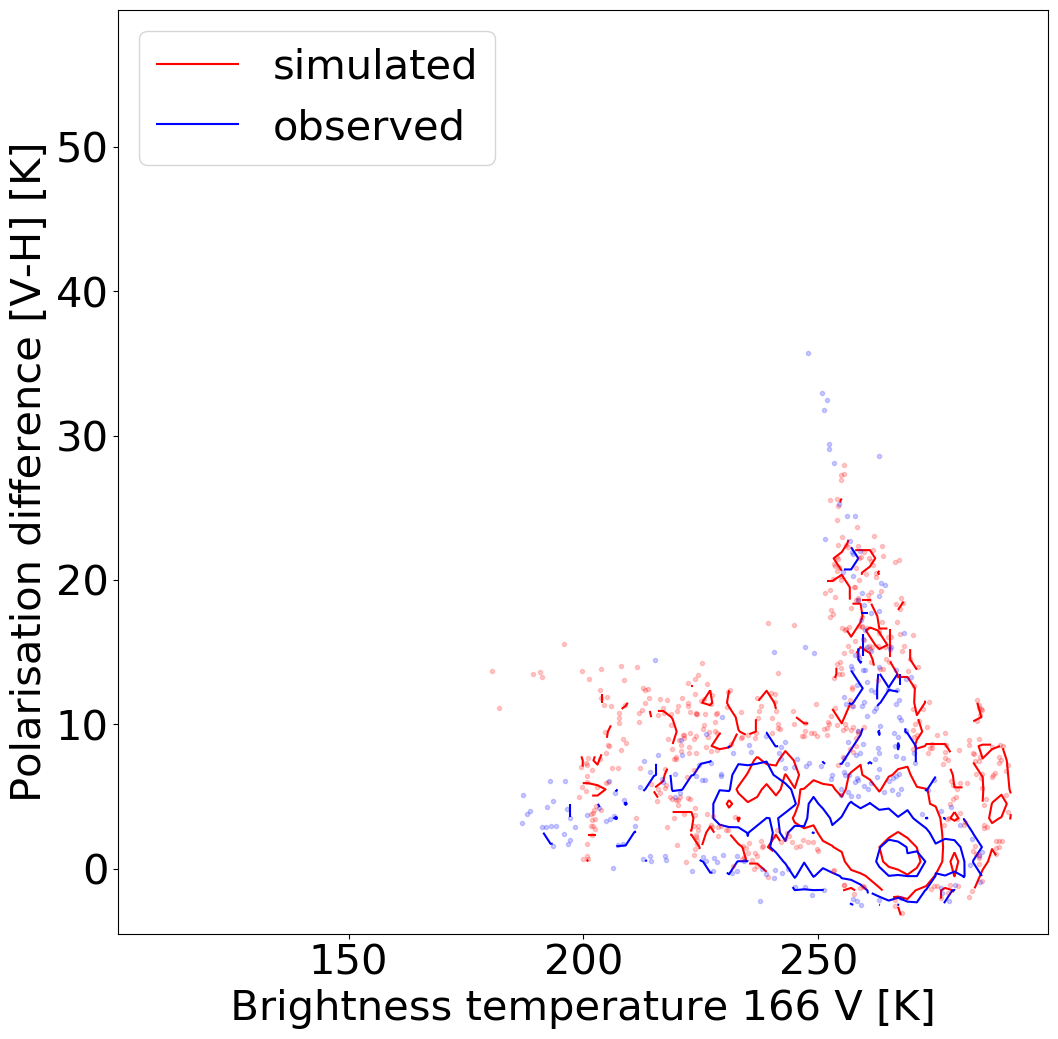
\includegraphics[height =35mm]{Figures/hist2d_gmi_45-60_land.png}
	\end{subfigure}
	\begin{subfigure}{.24\textwidth}
		\caption{Water}
		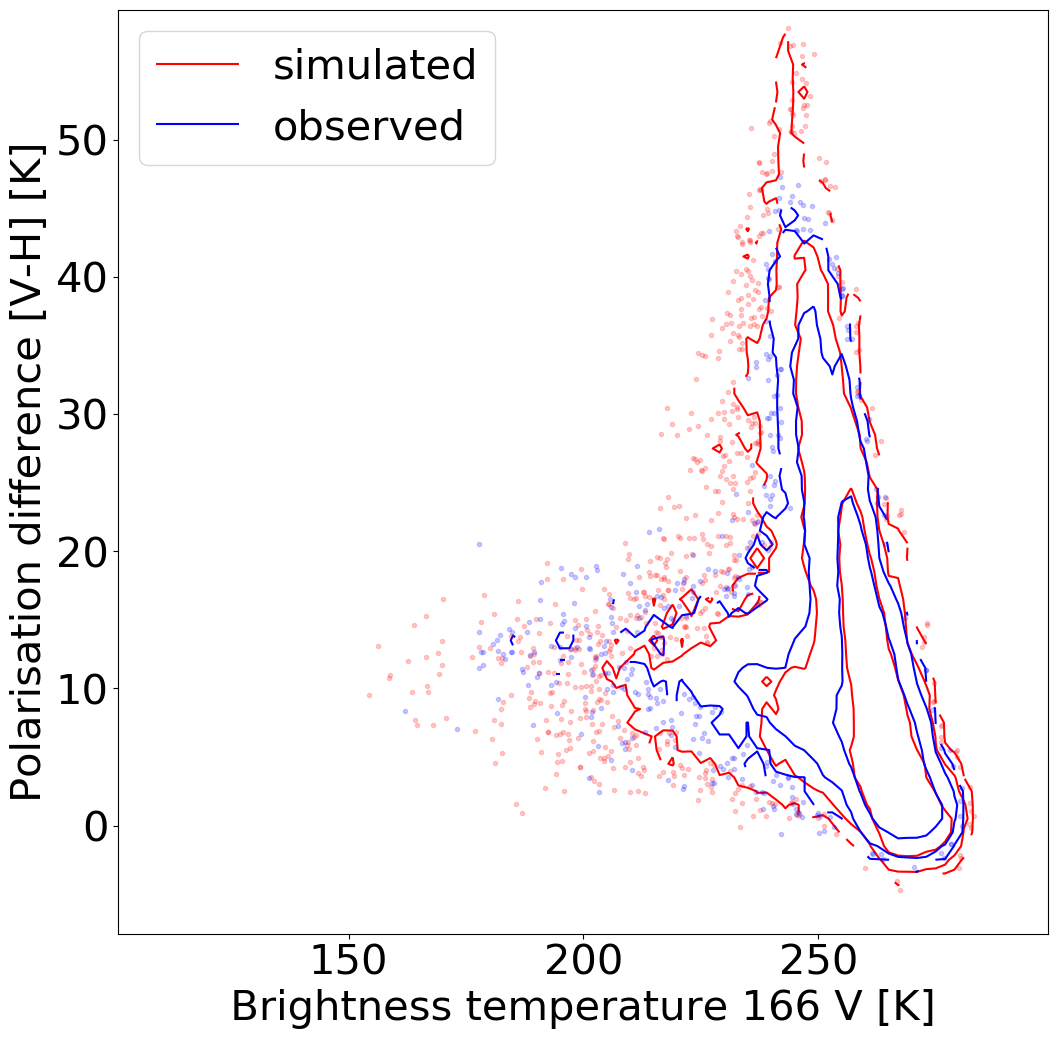
\includegraphics[height = 35mm]{Figures/hist2d_gmi_45-60_sea.png}
	\end{subfigure}
	\begin{subfigure}{.24\textwidth}
	\caption{Snow}
	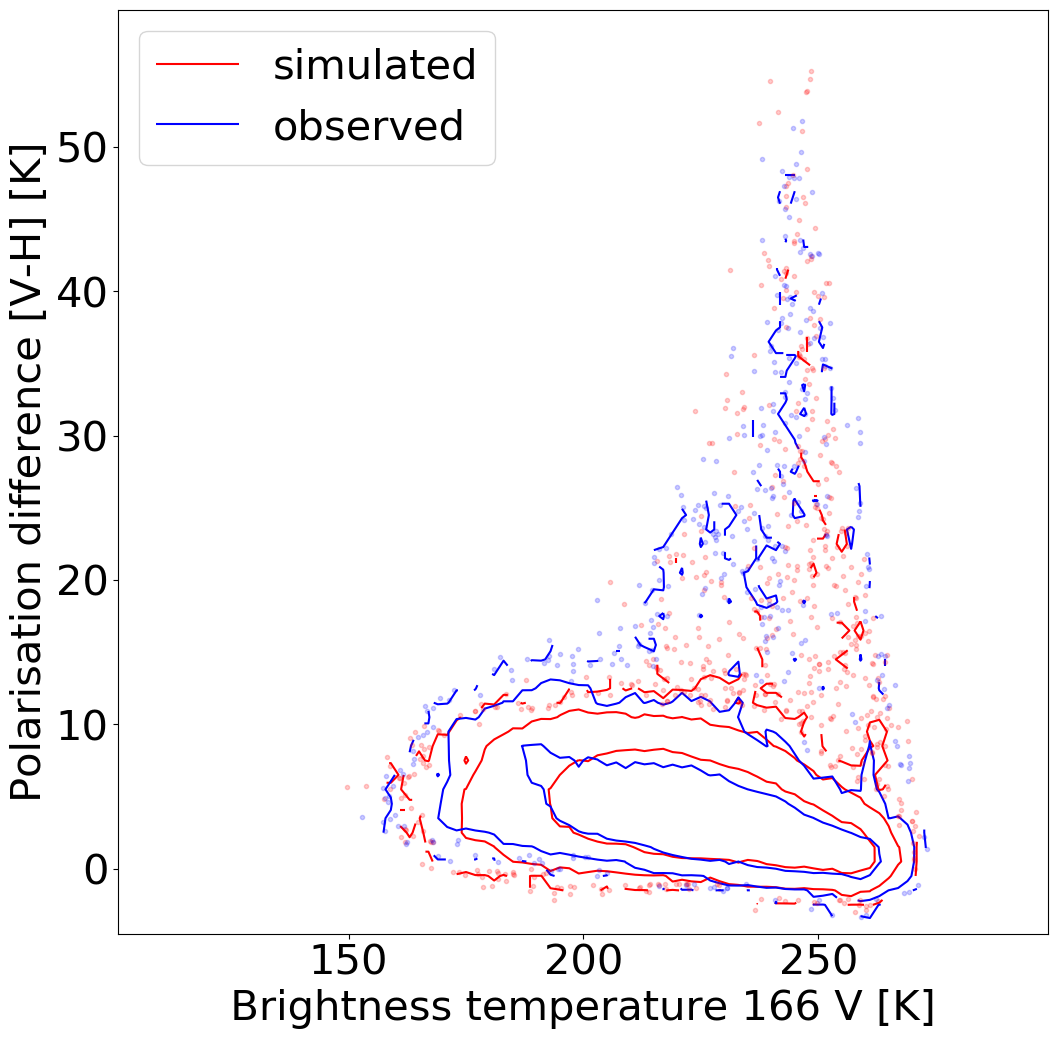
\includegraphics[height = 35mm]{Figures/hist2d_gmi_45-60_snow.png}
\end{subfigure}
\begin{subfigure}{.24\textwidth}
	\caption{ Sea-ice}
	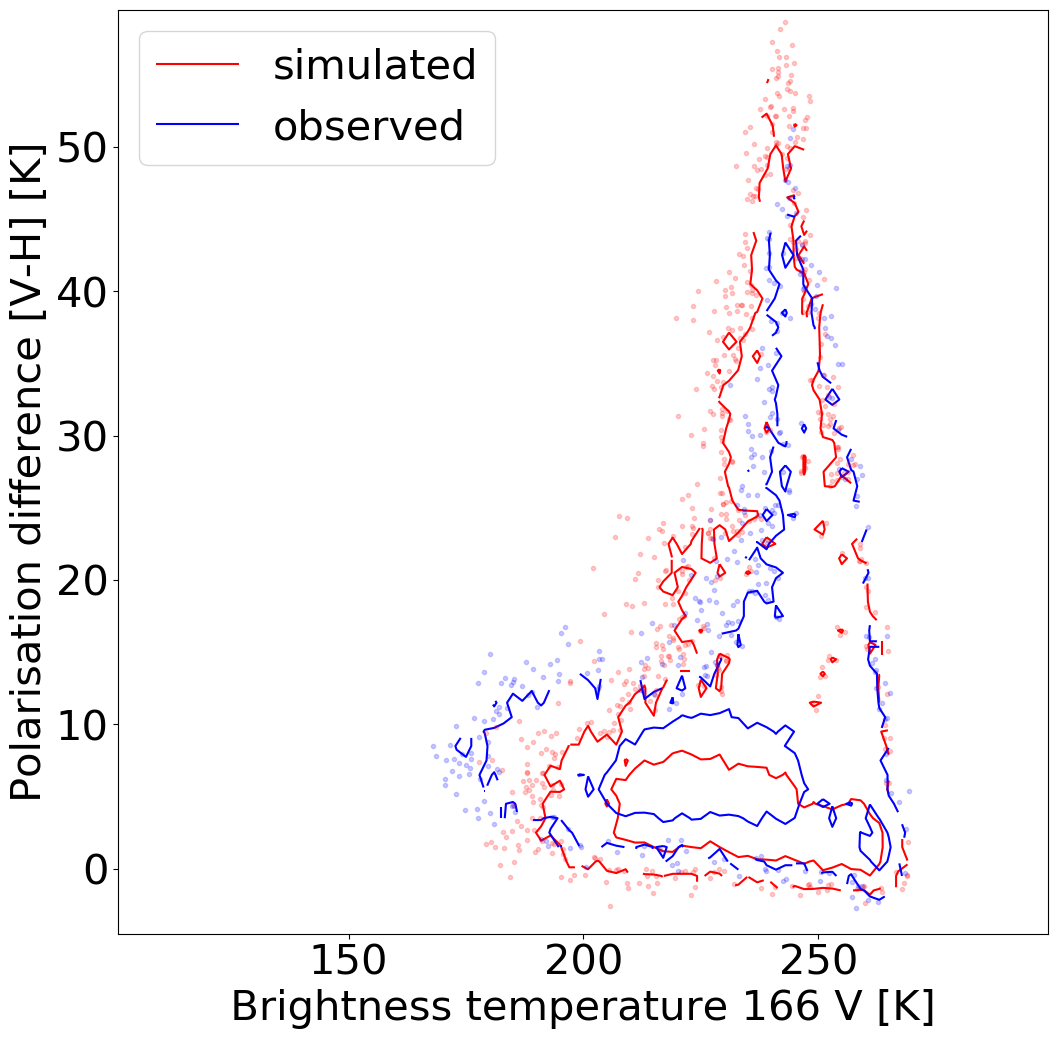
\includegraphics[height = 35mm]{Figures/hist2d_gmi_highlat_sea-ice.png}
\end{subfigure}
	\label{fig:histogram_2d}
	\caption{Two-dimensional PDFs for the TB and PD for GMI 166\,GHz frequency. Figures (a)-(d) are for land, water, snow and sea-ice surface types respectively. The simulated GMI data is from Jan 2009, while GMI measurements are from Jan 2020.}
\end{figure*}

In order to verify that the data in the training database covers the actual measurement space, the measured and simulated TB from GMI are compared statistically. Figure~\ref{fig:histogram_2d} shows the polarisation difference (PD) and TB histograms from 166 GHz for different surface types. The PD is defined as difference between V and H polarisations. The effect of including particle orientation using the scheme of \citep{baralakas:intro:21} indeed looks promising to mimic the effect of hydrometeor interaction.
Over both sea-ice and snow, the PDs are mostly positive as a consequence of hydrometeor scattering, and the negative PDs arise from noise in clear-sky measurements. For all surface types, the variability of our simulations is higher than the GMI measurements, indicating that the simulations can cover the all possible range of conditions. This is important as we cannot expect the retrieval to provide a complete picture, if the training database covers the measurement range partially.

\subsubsection{Retrievals}

\begin{figure*}[t]
	\centering
	\begin{subfigure}{.54\textwidth}
		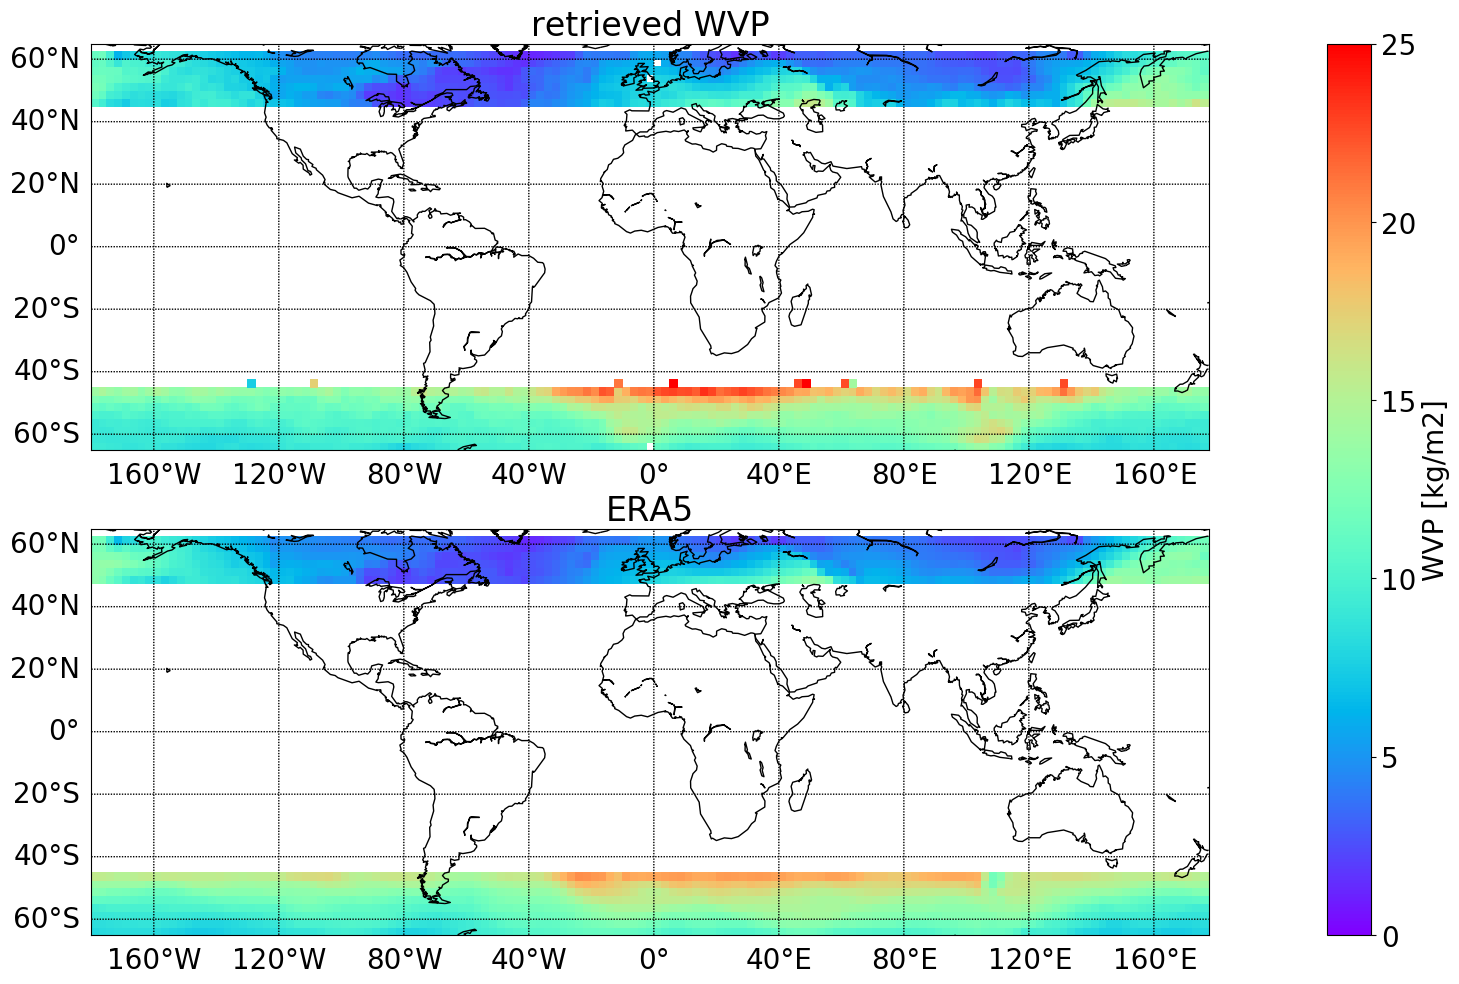
\includegraphics[height = 55mm]{Figures/WVP_spatial_jan2020.png}
	\end{subfigure}
	\begin{subfigure}{.34\textwidth}
	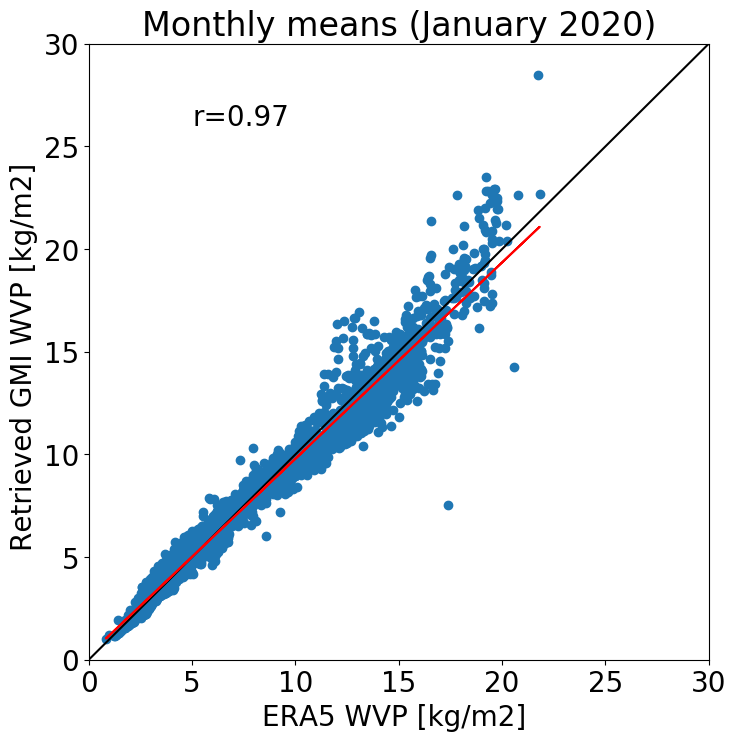
\includegraphics[height = 50mm]{Figures/WVP_scatter_monthlymean.png} 
	\end{subfigure}
	\caption{The spatial distributions (left) of monthly means estimated from retrieved WVP and ERA5 WVP. The data is for January 2020. The corresponding scatter between the two datasets is shown on the right. The red line is the line of best fit, while the black indicates the perfect fit.}
\end{figure*}


The QRNN algorithm described in sec~\ref{sec:qrnn} is applied to measured TB from GMI frequencies: 166 V\,GHz, 166 H\,GHz, 183$\pm$3\,GHz and 183$\pm$7\,GHz, to retrieve the corresponding WVPs. Two-metre temperature, latitude and surface type are also provided as auxiliary information. In order to compare the retrieved WVP with ERA5 total column wate rvapour (TCWV), the retrievals are re-gridded to 2.5$^{\circ}$ resolution. A comparison of the monthly means from both datasets is displayed in fig~\ref{fig:wvp_scatter}. The correlation between the monthly means between the two datasets is 0.97. 



\subsection{Work Flow}

The main task of project the first part is to create as realistic and comprehensive retrieval databases as possible. These calculations would at least include a description of the footprint response and a variety of particle models. The ambition of the project is to add more details which can reproduce the both high and highly variable emissivities over the sea-ice and snow regions.  It would also be important to include details of the particle orientation
and impact of footprint remapping. The overall retrieval setup will be similar to as employed in studies like \citep{eriksson:towar:20, ekelund:using:20}. The main output of the retrievals would be WVP, but indirect results like high resolution retrieval of sea-ice concentration (SIC) and liquid water path (LWP) would be an added advantage.


\subsection{Work packages}

\begin{figure*}[t]
	\centering
	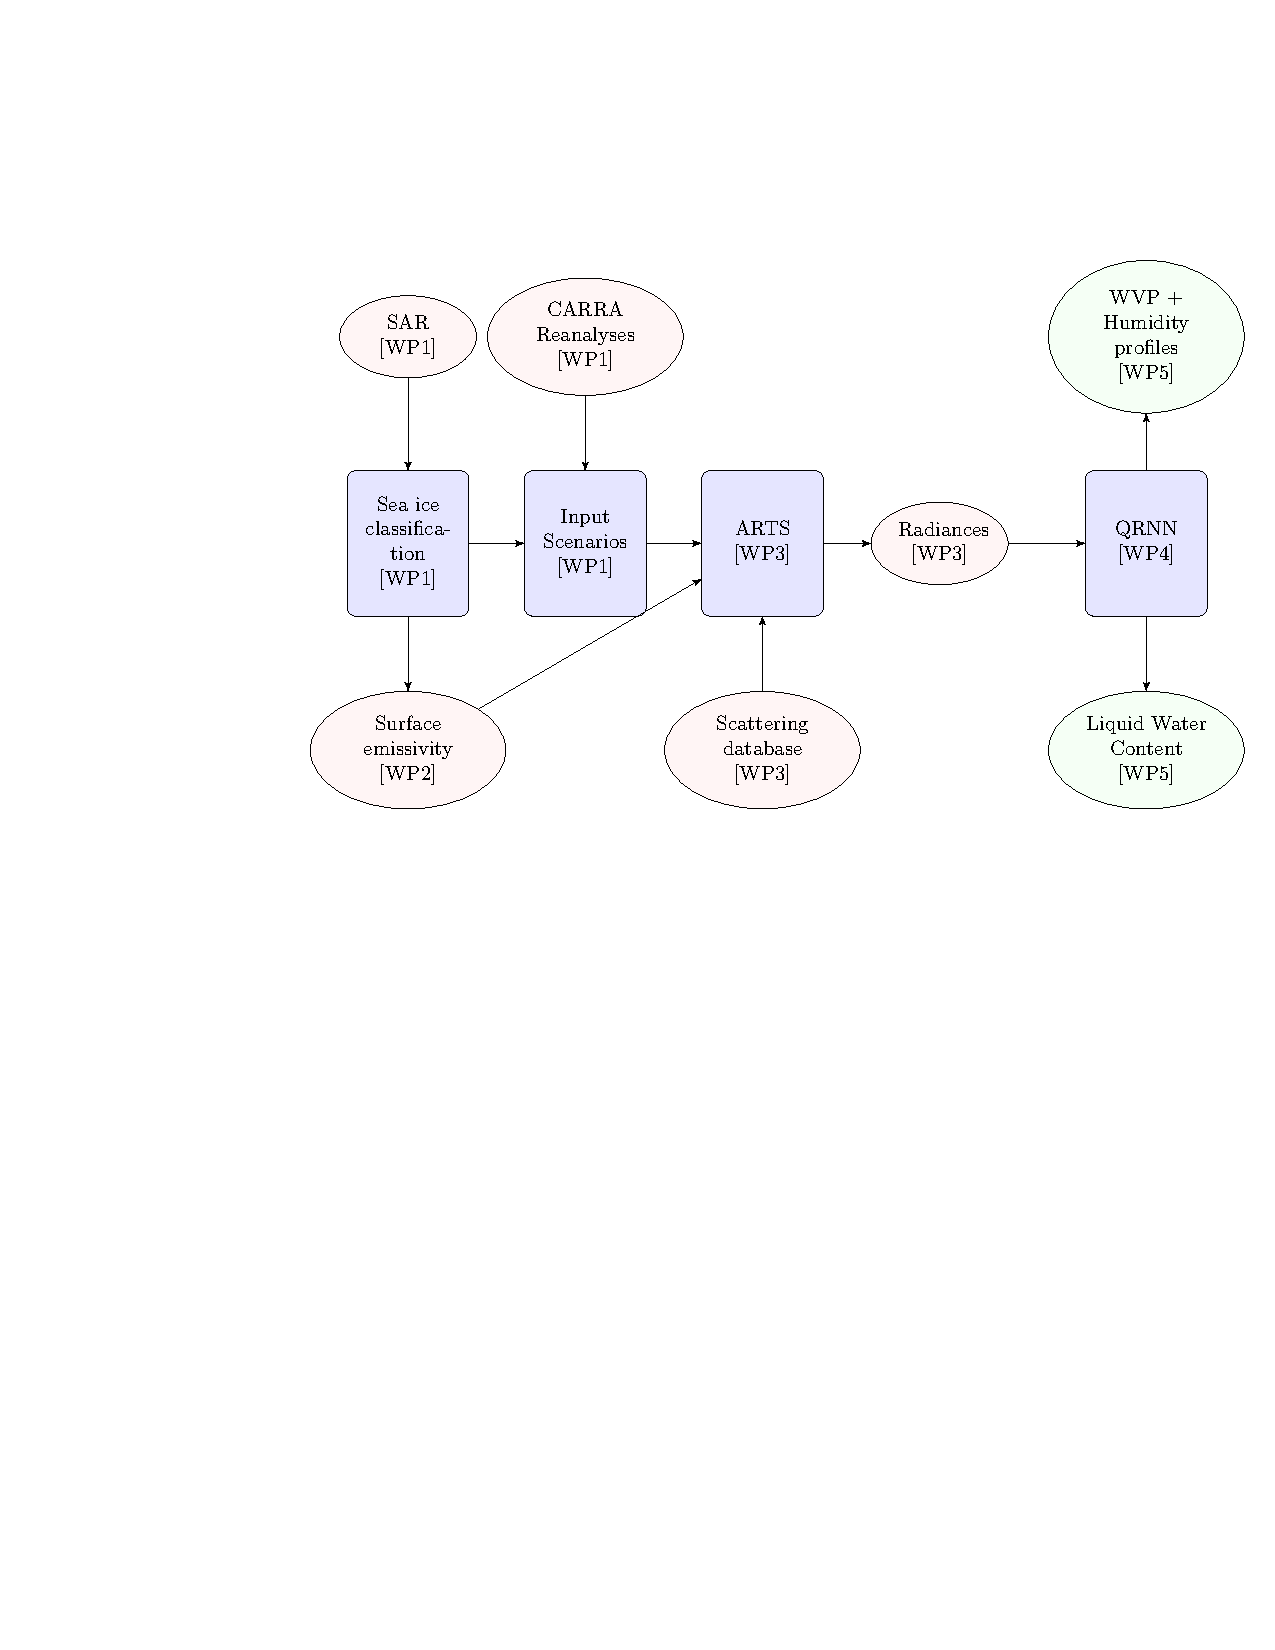
\includegraphics[trim=140 290 20 100,clip,height = 90mm]{flowchart.pdf} 
	\caption{Flowchart displaying schema of the proposed retrieval system.}
	\label{fig:flowchart}
\end{figure*}

\subsubsection{Part A: MW radiative transfer modelling system}

\subsubsection*{WP A1: Basic atmospheric scenarios}

As pointed out in \citet{eriksson:towar:20}: The input to the simulations can
be obtained from atmospheric models providing a sufficiently detailed
description of hydrometeors \citep[e.g.][]{wang2017statistical}. This approach
relies on that the model mimics reality with sufficient accuracy, as it
represents the a priori for the retrievals. Another option is to base the
simulations directly on observations as far as possible. In this study, we shall base the input to simulations through model observations. Over two sub-domains of Arctic, regional reanalyses performed with HARMONIE-AROME system at 2.5\,km resolution are available. This additional reanalyses available for European Arctic have improved parametrisations and extensive use of satellite data not previously used. Additionally, another option could be to use ICON model
(\url{www.mpimet.mpg.de/en/science/models}) that our colleagues in Hamburg have direct access to. 
The output of this work package would be a broad set of 3D atmospheric scenarios to be used as input to the radiative transfer simulations.

\subsubsection*{WP A2 : Emissivity model}

An important step to accomplish this project task is the estimation of the surface emissivity spectra over a multitude of surface types. Presently we use an empirical snow and sea-ice emissivities, but in this work package we would work attempt to utilize OEM based inversion to extract microwave emissivity spectra from TB, particularly for sea-ice surface types. 

\todo{how to describe OEM retrievals, } 
	
\subsubsection*{WP A3 : Database creation}
%	
This WP covers to launching and supervising the batch radiative transfer calculations (by ARTS).
Initially some time will be needed to implement the scripts needed for the basic calculations,
to add jobs to the calculation cluster and the post-processing needed. Simulations covering channels at 89, 166, 183 and 325 GHz will be made. A number of scan angles, between nadir and swath edge, will be covered. The overlapping antenna footprint of all frequencies will be explicitly simulated so that it is feasible to retrieve parameters at a finer scale than individual antenna beams. To generate the antenna pattern at a the desired frequency, a number of pencil beam radiative transfer calculations will be performed to incorporate both along-track and across-track sampling.
 
The WP output shall be batches of simulated radiances that are put into one or several retrieval databases. 

\subsubsection*{WP A5 : Retrieval setup}
%
The package for QRNN is already available as a part the Typhon software package \citep{lemke:2020:typho}. The implementation of the retrieval algorithm shall be relatively straightforward but the challenge would be to find the best performing neural-network architecture so as to achieve the best model performance. Besides, it would also be important to test the sensitivity of various auxiliary data to the retrieval performance. In order to run the retrievals, we shall make use of the Chalmers central computational cluster (C3SE).

\subsubsection*{WP A6 : Retrievals}
%
The use of the retrieval database shall we made without introducing any re-mapping between the different footprint sizes. All footprints inside a region would be used as input, and the database generation will mimic this. This approach will make much better use of
the spatial information provided by the overlap of AWS footprints. This has been demonstrated using 2DVAR in \citep{duncan:onthe:19}. But here we shall aim to achieve the same purpose by using QRNN. In fact, by doing this by a database (and not 2DVAR) we are not restricted to describe spatial correlations by covariance matrices and the QRNN version should be even more advantageous.

\subsection{Part B: Analysis and application}

The main tasks of this work package are to understand the quality of the retrievals, and pave way for their optimal use. The existing WVP retrievals from polar orbiting satellites do offer well sampled datasets, but the skill of the datasets is highly variable over different atmospheric and surface conditions. For example, in central Arctic, the differences between monthly means over summer months can be as high as 30\% \citep{crewell:2021:asyst}. Since in this project we aim to solve the retrieval issues associated with the ever complex and changing surface characteristics of sea-ice, a detailed assessment would be expected to improve the applicability and future retrieval algorithms.

\subsubsection*{WP B1 : Assessment with available products}

In order to evaluate the quality of the retrievals, in this work package, we shall aim at reviewing the performance with other available products. In this study a thorough investigation with the available \textit{in-situ} data, satellite products and reanalysis would be made. Firstly, direct comparisons with radio-soundings or data from flight campaigns would be used to estimate the accuracy of the product and reveal the uncertainties on finer scales.  Direct comparisons with other satellite products from AMSR \citep{gomez:2020:impro} will also made, but owing to different orbit characteristics of other satellite based products (e.g. from IR), statistical comparison is more appropriate. Time series of daily and monthly means, and the probability distribution functions (PDFs) of the retrievals would be analysed.

Here it would also be important to analyse the accuracy over seasons and different surface types: open water and sea-ice regions being the most important.

\subsubsection*{WP B2 : Applications}

\todo{0.3 page}

\subsubsection*{WP B3 : Additional Retrievals}

The MW emissivity spectra has characteristic features important to retrieve the sea-ice concentration. The high resolution emissivity retrievals can additionally be post-processed to generate estimates of SIC. The post-processing simply involves matching the 1D-VAR emissivity estimates over sea-ice to a pre-computed catalog of mean emissivity spectra. Infact, validation of the SIC against other available products like MiRS (Microwave Integrated Retrieval System) based operational cyrogenic products (\url{https://www.star.nesdis.noaa.gov/mirs/highresolutionv.php}) can also serve as an indirect validation of the emissivity retrievals.

\todo{catalog ?} 


\subsection{Risk Assessment}
0.5 page

\section{Collaborations}

In order to receive feedback on the retrieval database, we would closely collaborate with group working on WVP retrievals at University of Bremen to cover the analysis and validation aspects. Additionally, a contact with the group of Prof. Susanne Crewell would be also be useful for validation purposes. Their group is operating the MiRaC airborne sensor (a combined radar and radiometer) during polar flights (Mech et al., 2019).

\todo{ECMWF assimilation?}

\section{Staff situation}
\label{sec:staff}
%
Inderpreet Kaur (IK) started as a postdoctoral researcher in the division during March 2020.  She is presently working with both millimetre (mm) and sub-millimetre (mm) data for retrieval of atmospheric ice, and is interested in machine learning techniques for retrieval applications. During the project period, she shall spend almost 100\,\% of her time the project. 

Patrick Eriksson (PE) is a professor, .... time contribution??

Luisa Ickes (LI) started as an assistant professor during Jan 2020, and  general field is atmospheric modelling and the special research interests are the Arctic region and clouds in general. She will provide expertise in cloud physics, both when generating training data and evaluating retrievals.

Leif Eriksson (LE) is group leader for the research group Radar Remote Sensing. His research is aimed at development of methods to make measurements of land and ocean with radar data. In this project, his expertise is sought on the use of synthetic aperture radar (SAR) observations to identify sea ice concentration.

\section{Satellite data}
%
All satellite data of concern will be publicly available, as coming from
operational weather sensors.

{\footnotesize
	\bibliography{j_abbr,refs_pe1,references}
}
\end{document}
